\section{Corpus Processing}
\subsection{Levels of Linguistic Analysis}
There are several levels at which \textbf{linguistic analysis} can be performed, as shown in Figure~\ref{fig:linguistic_analysis_levels}.
\begin{figure}[!hbtp]
	\centering
	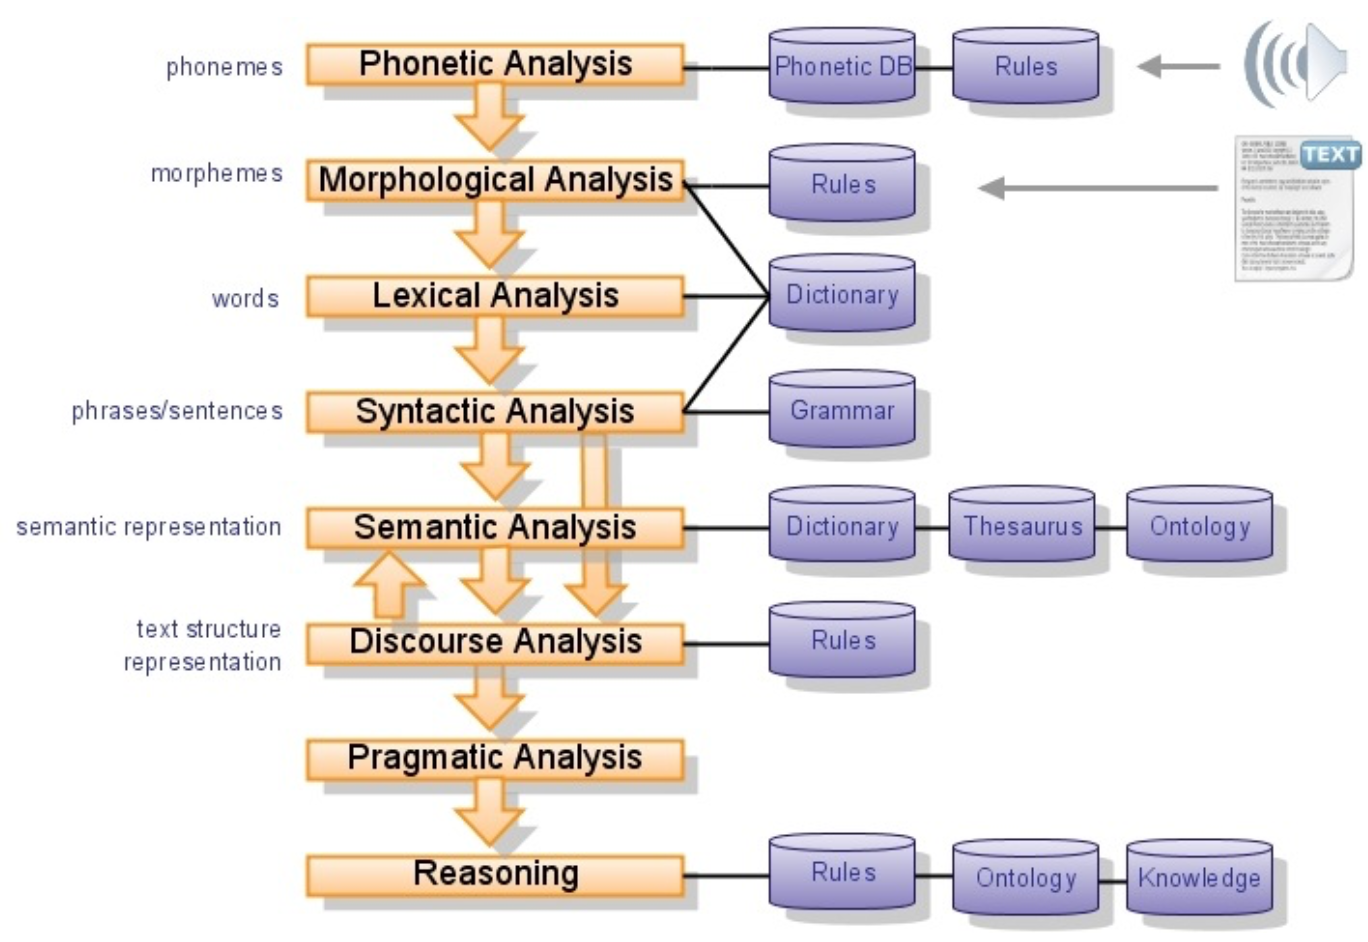
\includegraphics[width=\textwidth]{img/linguistic_analysis_levels}
	\caption{Different levels of linguistic analysis}
	\label{fig:linguistic_analysis_levels}
\end{figure}


\subsubsection{Phonetic Analysis}
\begin{mydef}[Phoneme]
	\textbf{Phonemes} are the \emph{smallest distinctive units} of a language.
	They are combined to form \emph{words}, and are abstract representations of \emph{speech sounds} or \emph{phones}.
\end{mydef}

\subsubsection{Morphological Analysis}
\begin{mydef}[Morpheme]
	\textbf{Morphemes} are the \emph{smallest meaningful units} of a language.
	They are abstract entities expressing \emph{semantic concepts} and \emph{grammatical features}.
\end{mydef}
There are essentially two types of \textbf{morphological variations}:
\begin{itemize}
	\item \textbf{Inflections}, which are \emph{grammatical} adaptations of a word in a particular \emph{syntactic context}, such as \emph{conjugation} or \emph{subject verb agreement}.
	\item \textbf{Lexical variations}, which can be \begin{itemize}
		\item \textbf{Derivations}, i.e. adding a \emph{bound morpheme} (affix) to a \emph{derivational base}; a derived form can become the base of a future derivation.
		\item \textbf{Compositions}, i.e. joining multiple base forms together.
	\end{itemize}
\end{itemize}

\subsubsection{Lexical Analysis}
\textbf{Lexical analysis} is concerned with analysing \emph{words}, for example by extracting \emph{lemmas} or assigning a \emph{part-of-speech} tag.
\begin{mydef}{Lemma}
	A \textbf{lemma} is the \emph{canonical form} of a word.
\end{mydef}

\begin{mydef}{Part-of-Speech}
	A \textbf{part-of-speech} is a \emph{grammatical category} identifying the \emph{nature} and/or \emph{syntactic function} of a word.
\end{mydef}

\subsubsection{Syntactic Analysis}
In \textbf{syntactic analysis}, the goal is to build a \emph{parse tree} of a sentence.
These parse trees represent the full \emph{structure} and the \emph{connection} between the different parts of a sentence.

\subsubsection{Semantic Analysis}
Building parse trees is potentially \emph{ambiguous} on a semantical level.
\textbf{Semantic analysis} allows us to distinguish between syntactically different (but correct) intepretations of a same sentence.

\subsubsection{Higher Levels of Analysis}
\begin{itemize}
	\item \textbf{Discourse analysis} is concerned with the analysis of text/speech beyond single sentences/utterances, by looking at \emph{relationships} between various sentences and paragraphs.
	\item \textbf{Pragmatic analysis} performs a \emph{reinterpretation} of text, to go \emph{beyond} the \emph{literal meaning}.
	\item \textbf{Reasoning}.
\end{itemize}

\subsection{Corpus Processing}
\subsubsection{Corpus Types and Properties}
\begin{mydef}[Corpus]
	A \textbf{corpus} is a \emph{large} body of linguistic evidence typically composed of \emph{attested language use}.
\end{mydef}
Corpora are considered the \emph{raw fuel} of computation linguistics.

A corpus should have the following properties:
\begin{itemize}
	\item \emph{machine-readable}: necessary for the computational aspect, or for performing quantitative analysis;
	\item preferably \emph{authentic texts} including transcripts of spoken data;
	\item ideally \emph{sampled} to be \emph{representative} of a particular language and/or specific task;
	\item \emph{large};
	\item \emph{well-organised} and \emph{well-formatted}.
\end{itemize}

There are various \emph{types} of corpora:
\begin{itemize}
	\item A \textbf{reference corpus}, which should be \emph{large}, \emph{balanced} and \emph{representative}.
	It is designed to provide comprehensive information about a language, including relevant varieties: spoken, written, \dots
	\item A \textbf{specialized corpus} covers a \emph{specific aspect} of the language: one theme, one author, one genre, \dots
	\item A \textbf{monitor corpus} is a \emph{continuously updated} (as opposed to \emph{static}) corpus with new materials.
	\item A \textbf{multilingual corpus} is useful when \emph{translating} between various (forms of) languages.
	\textbf{Parallel corpora} contain text in one language with their translation in another or more languages.
	These translations are often combined with alignment techniques in order to form an \textbf{aligned corpus}.
\end{itemize}
Corpora can be \emph{oral}, \emph{written} or even \emph{multimedia}.

\subsubsection{Corpus Annotation}
\begin{mydef}[Annotation]
	\textbf{Annotation} is the practice of adding \emph{interpretative}, \emph{linguistic} information to an electronic corpus of spoken and/or written language data.
\end{mydef}
These annotations
\begin{itemize}
	\item can be \emph{manual} or \emph{automatic},
	\item contain \emph{metadata} making some type of linguistic information \emph{explicit} (hard to do),
	\item access \emph{deeper linguistic levels} which are not directly accessible through the surface text,
	\item \emph{improve} the corpus \emph{usability}
\end{itemize}

There are several levels of annotation:
\begin{itemize}
	\item \textbf{orthographic annotation}: markup, italics;
	\item \textbf{phonetic/phonemic annotation}: transcription of speech sounds;
	\item \textbf{prosodic annotation}: syllables, intonation contours;
	\item \textbf{morpho-syntactic annotation}: parts-of-speech, grammatical tagging;
	\item \textbf{syntactic annotation}: constituency parsing, dependency parsing;
	\item \textbf{semantic annotation}: entities, word meaning, predicates;
	\item \textbf{discoursal annotation}: anaphora and coreference resolution.
\end{itemize}

\subsubsection{Corpus Segmentation}
\begin{mydef}
	\textbf{Tokenization} is the task of chopping a given character sequence up into \textbf{tokens}.
	A \textbf{token} is an instance of a \emph{sequence of characters} in some particular document that are grouped together as a \emph{useful semantic unit} for processing.
	A \textbf{type} is the \emph{class} of all tokens containing the same \emph{character sequence}.
\end{mydef}
Tokenization is language-dependent: \emph{compound splitting} in Dutch or German, \emph{script segmentation} in Korean/Japanese/Chinese.

\textbf{Corpus segmentation} also needs to deal with \emph{punctuation}.
\begin{itemize}
	\item \textbf{Exclamation points} and \textbf{question marks} are almost always the end of a sentence.
	\item \textbf{Semi-colons} can be a separator of list elements or a sentence separator.
	\item \textbf{Periods} can be the end of a sentence, part of an abbreviation, or both.
\end{itemize}

\subsubsection{Word Stemming}
\begin{mydef}[Lemmatization]
	\textbf{Lemmatization} is a linguistically motivated approach relying on a \emph{vocabulary}, \emph{morphological dictionaries} and \emph{morphological analyzers} to return \textbf{lemmas}.
\end{mydef}

\begin{mydef}[Stemming]
	\textbf{Stemming} is a \emph{heuristic process}, often used in \emph{information retrieval}, that chops off the end of words to produce \textbf{word stems}.
\end{mydef}

\textbf{Lemmatization} and \textbf{stemming} try to \emph{reduce inflectional forms} or derivationally related forms of a word to an \emph{uninflected base form}.

\paragraph{Porter Stemming Algorithm}
The algorithm uses the following definitions/notations:
\begin{itemize}
	\item \(v\) denotes a \emph{vowel}, i.e. \(v \in \{\textnormal{A, E, I, O, U, Y}\}\), where Y should be preceded by a \emph{consonant}.
	\item \(c\) denotes a \emph{consonant}, i.e. anything that is not a \emph{vowel}.
	\item \(V\) is a sequence of \(n > 0\) \emph{vowels}.
	\item \(C\) is a sequence of \(n > 0\) \emph{consonants}.
\end{itemize}
Any word can then be represented as \([C](VC)\{m\}[V]\), where \([C]\) and \([V] \geq 0\) (note the square brackets also allowing \(n = 0\)) and \((VC)\) can be repeated \(m\) times.

\emph{Stemming rules} for removing a \emph{suffix} are as follows:
\begin{itemize}
	\item They take the form \((\textnormal{condition on \textbf{stem}}S_1 \to S_2)\). If the \emph{stem} satisfies a given condition and \(S_1\) is a suffix, then \(S_1\) is replaced by \(S_2\) (which can be empty).
	\item Rules are applied in 5 successive runs, where several rules are applied at each run, and each rule is evaluated until one matches, then the next run starts.
\end{itemize}

This algorithm tries to replicate a true \emph{lemmatization} of the input text.
Common \emph{approximations} are
\begin{itemize}
	\item \textbf{under-stemming}, which is the failure to group words having a shared meaning, or
	\item \textbf{over-stemming}, which is the grouping of words with no shared conceptual meaning.
\end{itemize}